\chapter{The Large Hadron Collider and the CMS experiment}

This work is based on data collected by the Compact Muon Solenoid (CMS) experiment, 
one of the four main experiments together with ATLAS, ALICE and LHCb exploiting the collisions 
provided by the Large Hadron Collider (LHC). A detailed description of the LHC and of the CMS 
experiment can be found in \cite{Evans:2006tq} and \cite{Chatrchyan:2008aa} respectively.

\section{The Large Hadron Collider}

The LHC and its experiments were built to explore the so called high energy frontier of particle physics and try to address fundamental questions of this field like the presence of a Higgs boson, the existence of supersymmetry or other new structures like extra dimensions or an additional quark families. All these phenomena don't have a well-defined energy range imposed by theory even though are expected to manifest at the TeV scale, therefore a proton-proton collider was considered to be the most suitable machine for such a task, allowing higher energies with current technologies and probing wider energy ranges at the same time exploiting the compositeness of the colliding particles.

The LHC is housed in the 27 km underground tunnel where the large electron positron collider (LEP) has been operating until its decommissioning which started in the year 2000. The tunnel is located under both French and Swiss territory in proximity of the CERN research facility. Before getting to the LHC protons are produced from hydrogen ionization and then accelerated through a chain of smaller accelerators, some of them dating back to the late 1950's. A schematic view of the CERN accelerators and their connection is depicted on Figure \ref{fig:cern_accelerators}. From the last element of this chain, the Super Proton Syncrotron (SPS), protons are injected in the LHC with an energy of 450 GeV in two separate beam pipes, one containing protons running clockwise, the other with protons running in the opposite direction. Protons are bent in their path with the aid of 1232 superconducting dipole magnets and focused by  superconducting magnets, while 16 superconducting radio-frequency (RF) stations provide the thrust to accelerate the two beams up to 7 TeV in steps of 0.5 MeV each turn. In order to maintain superconducting properties the magnet coils and the cavities the are cooled to 1.9 K by a complex cryogenic system that uses super-fluid helium as refrigerator. Using the RF cavities for accelerating the protons is possible only if the beam is not continuous but structured in bunches. By design the LHC is built to contain 2808 bunches of $10^{11}$ protons each, giving a bunch spacing of 25 ns.
%Due to space constraints both the beam pipes are encased in the same dipole and the proper magnetic field direction is achieved with a particular magnet design.  

\begin{figure}
\begin{center}
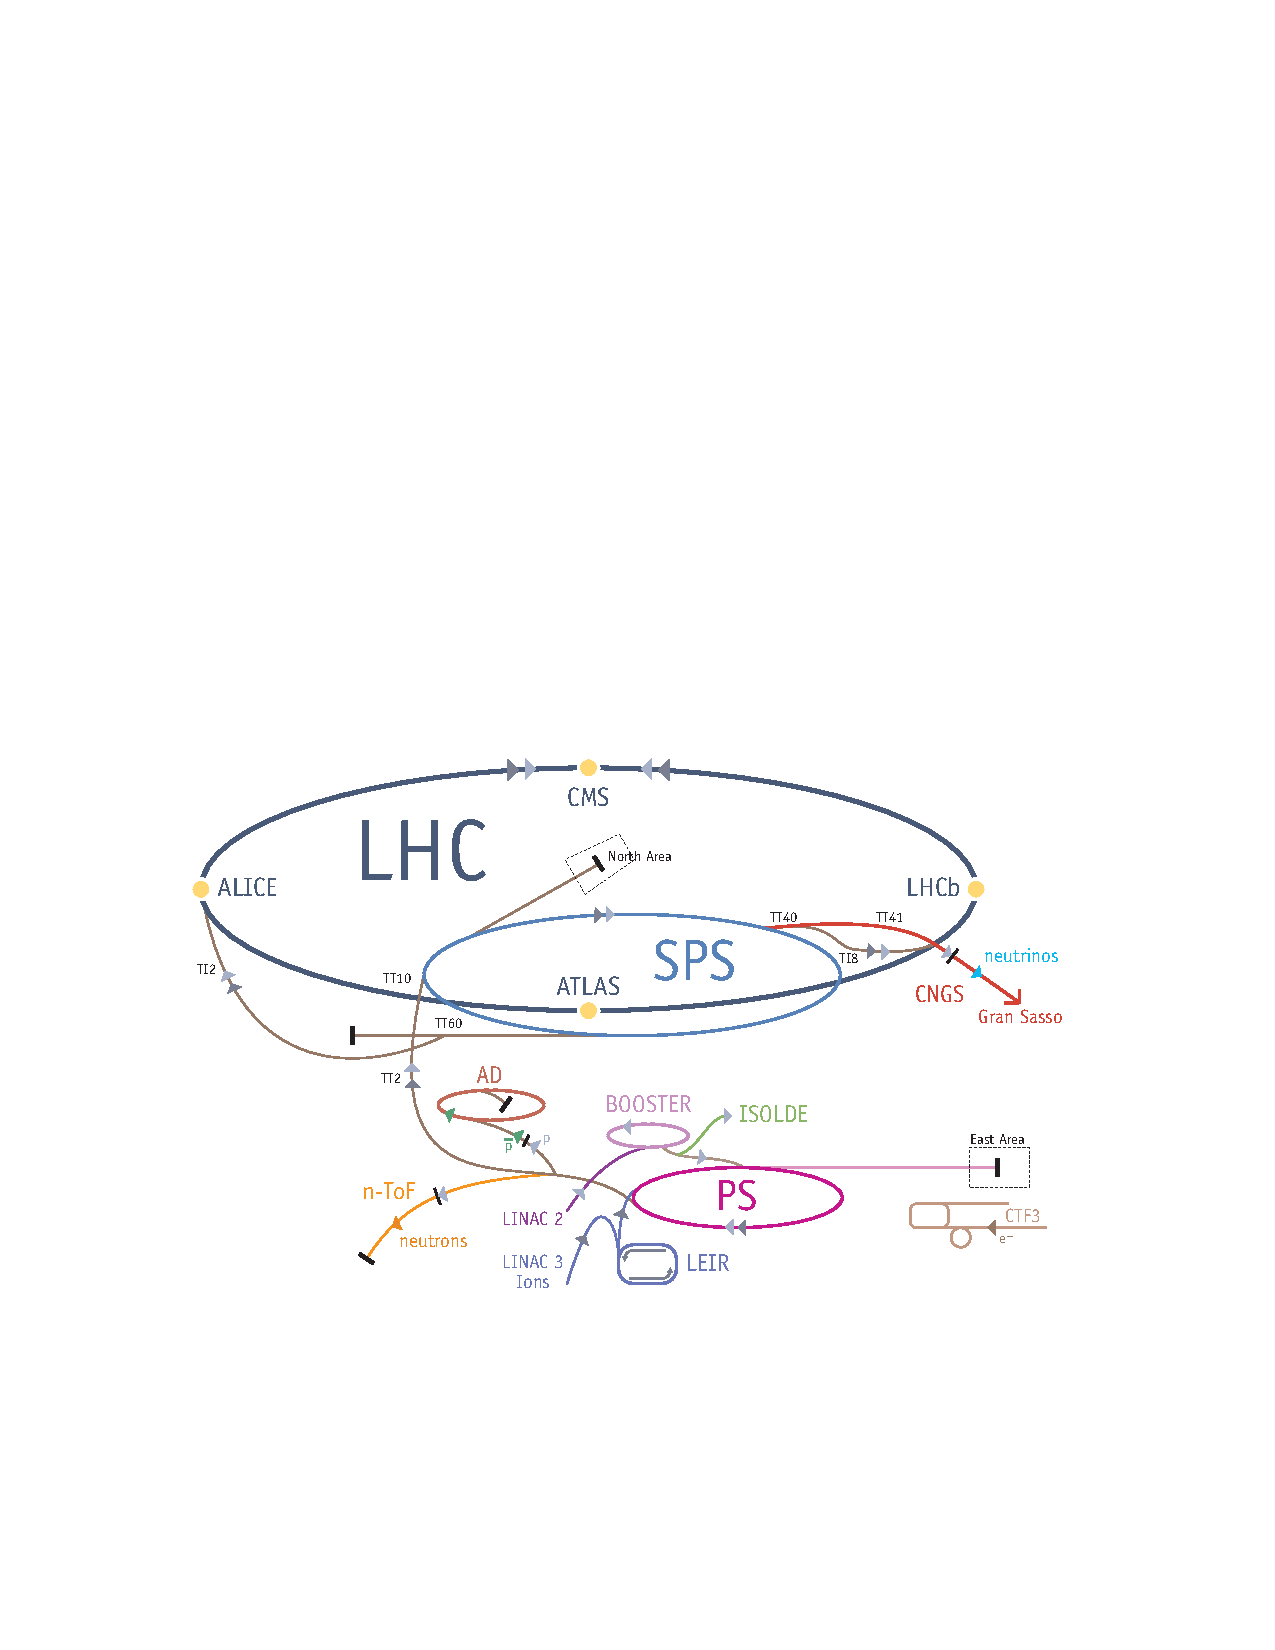
\includegraphics[angle=-0,width=0.8\textwidth]{2_LHC_and_CMS/pics/LHC.pdf}
\caption{Schematic view of the CERN accelerators and their connection
\label{fig:cern_accelerators}
}
\end{center}
\end{figure}

The LHC started its operation on 10 September 2008 and after only 9 days of operation a severe \emph{quenching} of about 100 dipole magnets, causing the release of around two tones of helium, forced the machine to stop and to reconsider the design figures of the machine. The main cause of the accident was found to be in some of the electrical connections between magnets. In year 2009, when the machine became again operational, a very careful ramp-up plan was scheduled, mainly focusing on the reduced energy of the beams, allowing for less current to flow in the steering magnets. The year 2010, after a careful ramp-up of the beam energies, saw the start of the LHC research program with collisions at a center of mass energy (\sqrts) of 7 TeV, half of the designed one. During 2010 and 2011 the machine commissioning went on along with physics runs improving the instantaneous luminosity and allowing for an increase in beam energy that took place in 2012, raising the beam energies to 4 TeV. Design values and achieved ones are summarized in table \ref{tab:lhc_figures}.

\begin{table}[h!]
   \centering
\begin{tabular}{c|ccccc}
\hline
Parameter & Design value&  Best value achieved \\ 
\hline
Beam energy   & 7 TeV & 4 TeV \\ 
Number of protons per bunch & 1.15$\times$10$^{11}$ & 1.5$\times$10$^{11}$ \\
Number of bunches & 2808 & 1368 \\
Crossing angle & 300~\si{\micro\metre} & 290~\si{\micro\metre} \\
Beam size & 17~\si{\micro\metre} & 20~\si{\micro\metre} \\
Emittance & 3.75 ~\si{\micro\metre} & 2.4~\si{\micro\metre}  \\
Peak luminosity & $10^{34}$~cm$^{-2}$s$^{-1}$ & 7.5$\times$10$^{33}$~cm$^{-2}$s$^{-1}$ \\
\hline
\end{tabular}
  \caption{Relevant LHC machine parameters. The design values are compared to the ones reached at the end of the 2013 operations.}
  \label{tab:lhc_figures}                
\end{table}


The instantaneous luminosity measures the number of particles per unit area per unit time available for collisions. For any given physics process the average number events is given by:

\begin{equation} 
	N_{ev} = \sigma\int\operatorname{\mathcal{L}}(t)\mathrm{d}t
	\label{eq:n_events}
\end{equation} 

Where $\sigma$ is the cross-section for such process. While the cross section is a constant of nature, the instantaneous luminosity can be entirely derived from accelerator figures:

\begin{equation} 
	\operatorname{{\cal L}}(t) = \frac{N_p^2 n_b f_{rev} \gamma }{4 \pi \epsilon_{n} \beta^*} F
	\label{eq:lumi}
\end{equation} 

where $N_p$ and $n_b$ are the number of protons per bunch and the total number of bunches respectively, $f_{rev}$ is the frequency of rotation, $\epsilon_{n}$ and $\beta^*$ describe the beam focusing at the interaction point, $\gamma$ is a relativistic factor and $F$ accounts for the crossing angle between the two beams. As it is possible to see from the previous table \ref{tab:lhc_figures}, even though the number of bunches has always been less than half the design value during all the running period, the peak instantaneous luminosity has only been 30\% lower than the design one. This result was achieved by increasing the number of protons in each bunch and increasing the focusing of the beams, at the price of increasing the average number of proton collisions per bunch crossing, the so-called \emph{pileup}. This effect is shown in figure \ref{fig:lhc_pileup} where is shown the peak number of interactions per bunch crossing in function of time as recorded by the CMS detector.

\begin{figure}
\begin{center}
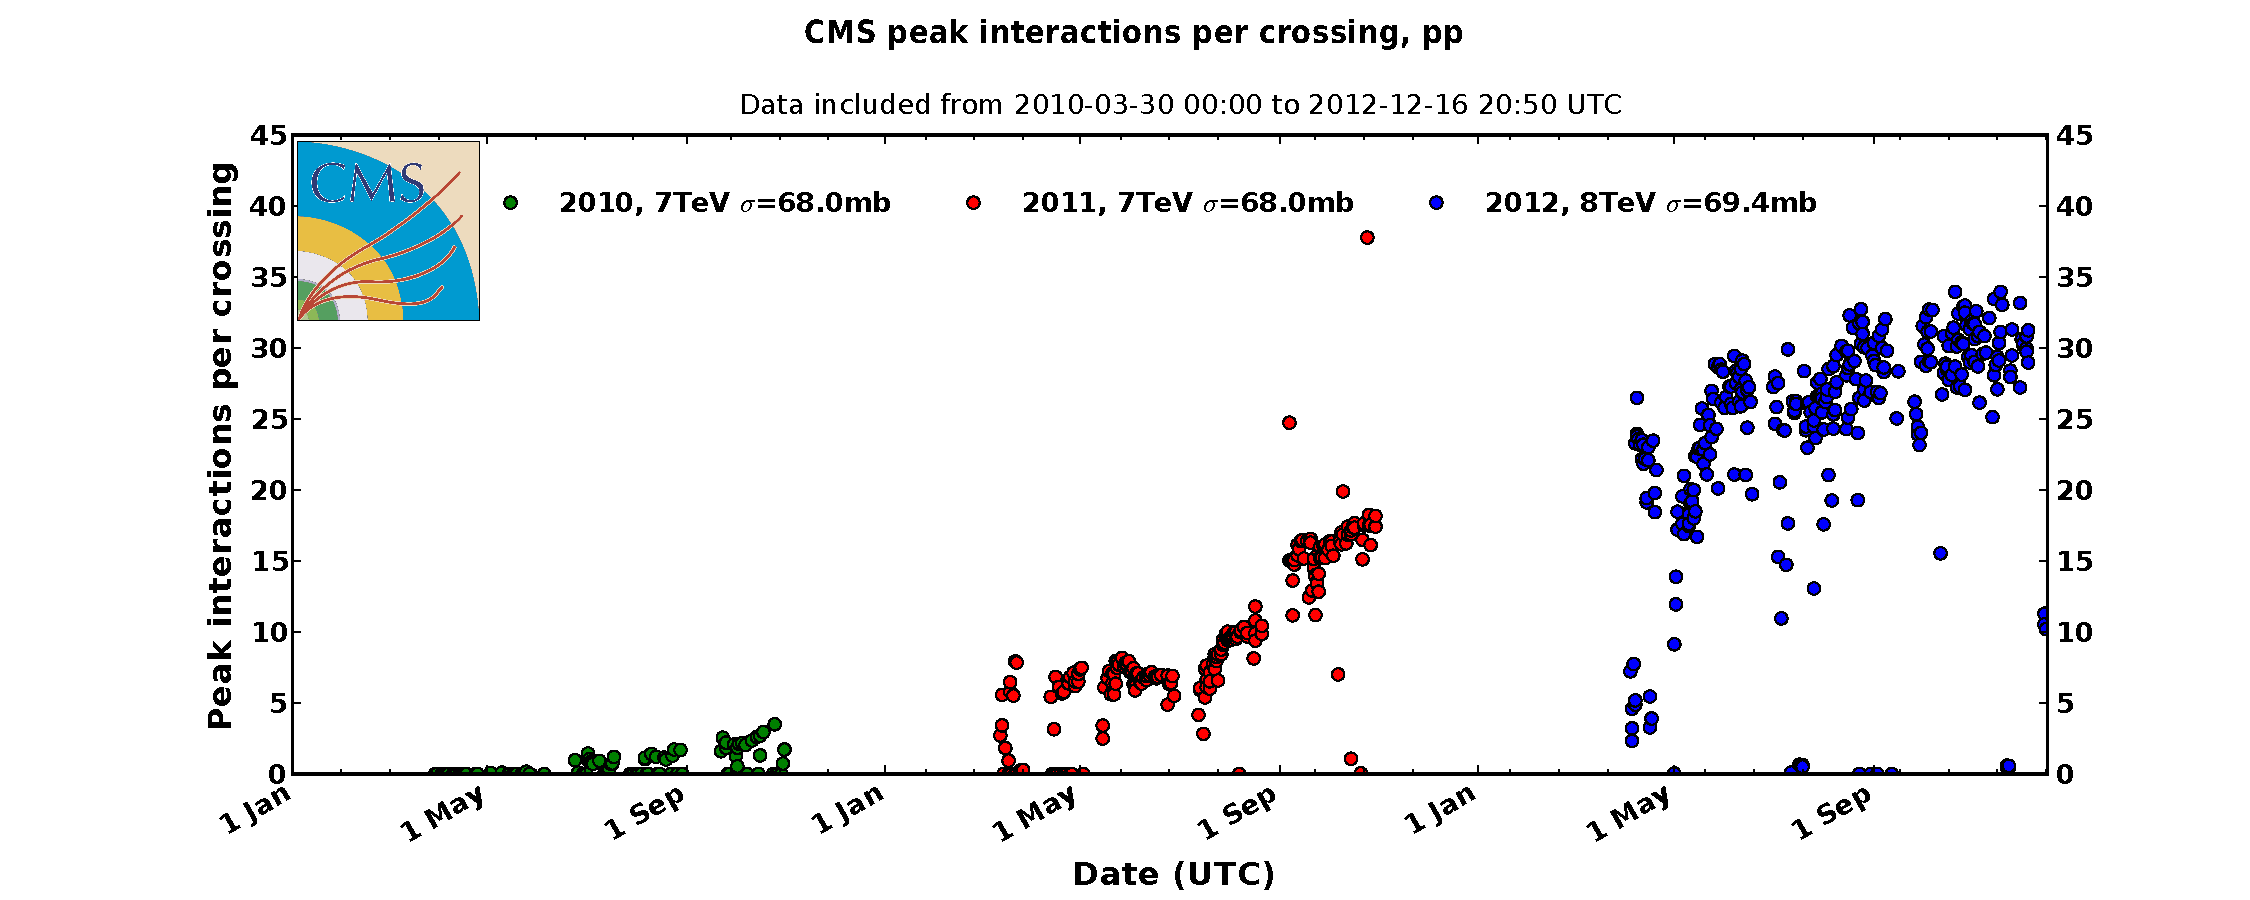
\includegraphics[angle=-0,width=\textwidth]{2_LHC_and_CMS/pics/peak_pu_pp.pdf}
\caption{Peak number of interactions per bunch crossing in function of time as recorded by the CMS detector
\label{fig:lhc_pileup}
}
\end{center}
\end{figure}

As can be clearly seen by equation \ref{eq:n_events}, the most important figure for physics searches is the integrated luminosity which is usually quoted as \L. During its operations LHC delivered 44.2~pb\Inv in 2010, 6.1~fb\Inv in 2011 and 23.3~fb\Inv at 8~TeV in 2012, the huge progress made by the accelerator can be clearly seen in figure \ref{fig:int_lumi}.

\begin{figure}
\begin{center}
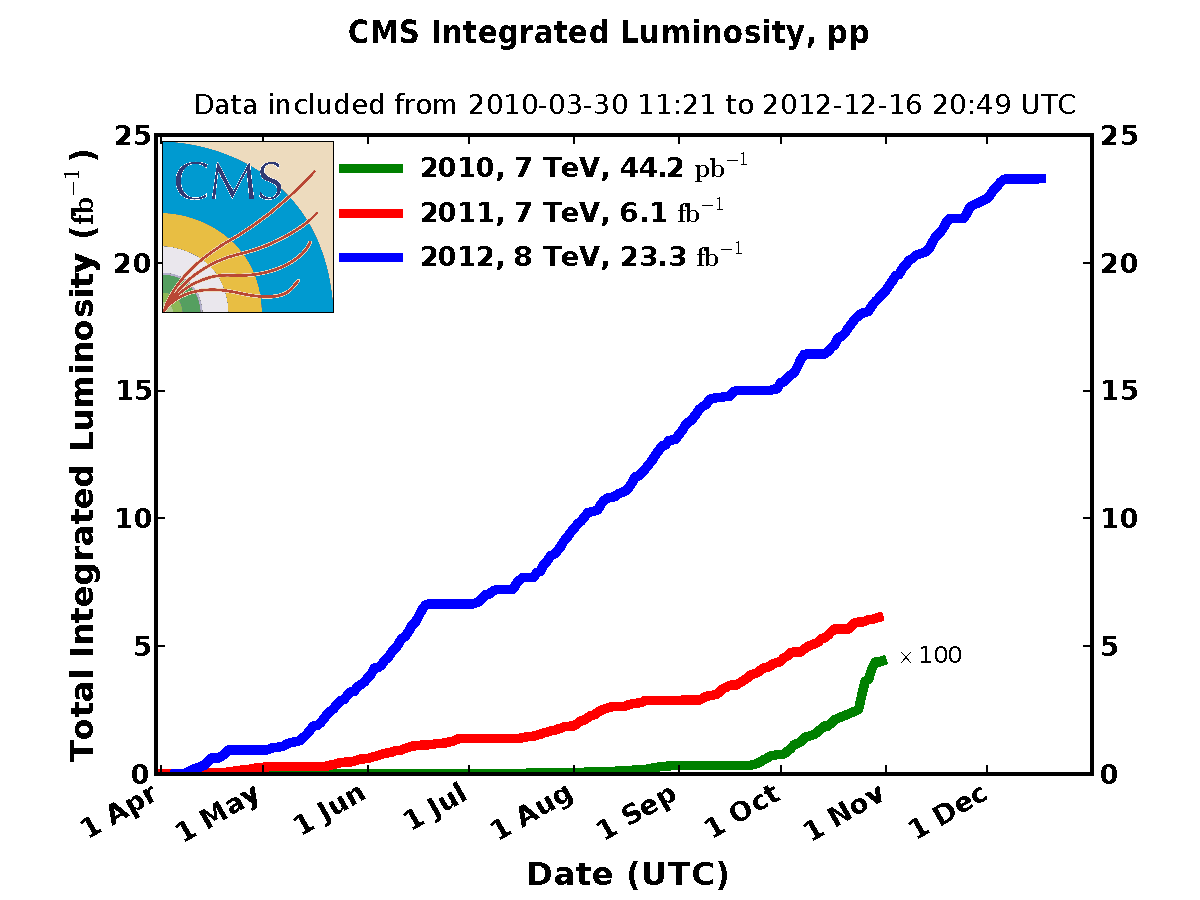
\includegraphics[angle=-0,width=0.8\textwidth]{2_LHC_and_CMS/pics/int_lumi.pdf}
\caption{Cumulative luminosity versus day delivered to CMS during stable beams and for p-p collisions. This is shown for 2010 (green), 2011 (red) and 2012 (blue) data-taking.
\label{fig:int_lumi}
}
\end{center}
\end{figure}


\section{The CMS detector}

The CMS detector is located at point 5 in the LHC tunnel, near the town of Cessy, France, between the Jura chain and the Leman lake.
 
The CMS detector, together with the ATLAS one, is one of the two multi-purpose detectors operating at the LHC. The prime task of the experiment is to probe the TeV scale looking for signs of new physics and to look for the Higgs boson, the only missing piece to the SM puzzle. At the same time the experiment was also designed to perform precision measurements in B-physics and in known standard model processes. A heavy-ion program is carried on as well to probe the rules of QCD at very high energies and matter densities, trying to reproduce an environment similar to the conditions of the universe few instants after the big bang.

To carry out such ambitious research program the detector was designed to meet some baseline requirements:
\begin{itemize}
\item Good muon identification and momentum resolution over a wide range of momenta and angles with di-muon mass resolution of ~1\% at 100~GeV.
\item Ability to identify the muon charge without any ambiguity for muons momenta below 1~TeV
\item Good charged particle momenta resolution and high tracking efficiency and resolution. This two figures are especially important for objects like \b-jets and taus, where isolated charged hadrons and displaced vertices play a fundamental role. A high tracking resolution also plays a key role in assigning the tracks to the belonging vertex mitigating the effect of pileup.
\item Good electromagnetic energy resolution, with di-photon invariant mass resolution of \~1\% at 100~GeV and wide geometric coverage with efficient photon and lepton isolation in high pileup conditions.
\item Hermetic hadronic calorimeter with fine transverse segmentation for good jet mass and missing transverse energy ($E_T^{miss}$) resolution. 
\end{itemize}

The total proton-proton cross section at 14~TeV is expected to be roughly 100~mb, with LHC design values it is therefore expected an average of 20 inelastic collisions for each bunch crossing, a value that was widely overcome in all the 2012 run. This number of overlapping events, also referred as \emph{pileup}, together with the short 25~ns bunch spacing pose stringent requirements on the resolution, granularity and latency of the different sub detector. It is in fact of primary importance to be able to resolve the overlapping vertices and assign their respective track, while still being fast enough to avoid overlapping of two different bunches in the same electronic output. A fast trigger system is also required to bring the event rate from \~40~MHz to \~100Hz which can be permanently stored.

In order to meet all these requirements CMS has been built with a 4~T NbTi superconducting solenoid magnet of 6~m of inner diameter. Inside the magnet a large silicon tracker, the largest of its kind, is housed to provide the inner tracking with the required resolution. Around the tracker, but still within the solenoid field a lead-tungstanate electromagnetic calorimeter (ECAL) and a brass-scintillating sampling hadron calorimeter (HCAL). Inside the 1.5~m of iron constituting the return yoke of the magnet four muon stations are housed. These muon stations consist in several layers of drift tubes or cathode strip chambers complemented by resistive plate chabers. A schematic view of a slice of the CMS detector is presented in figure \ref{fig:cmsdet}

\begin{figure}
\begin{center}
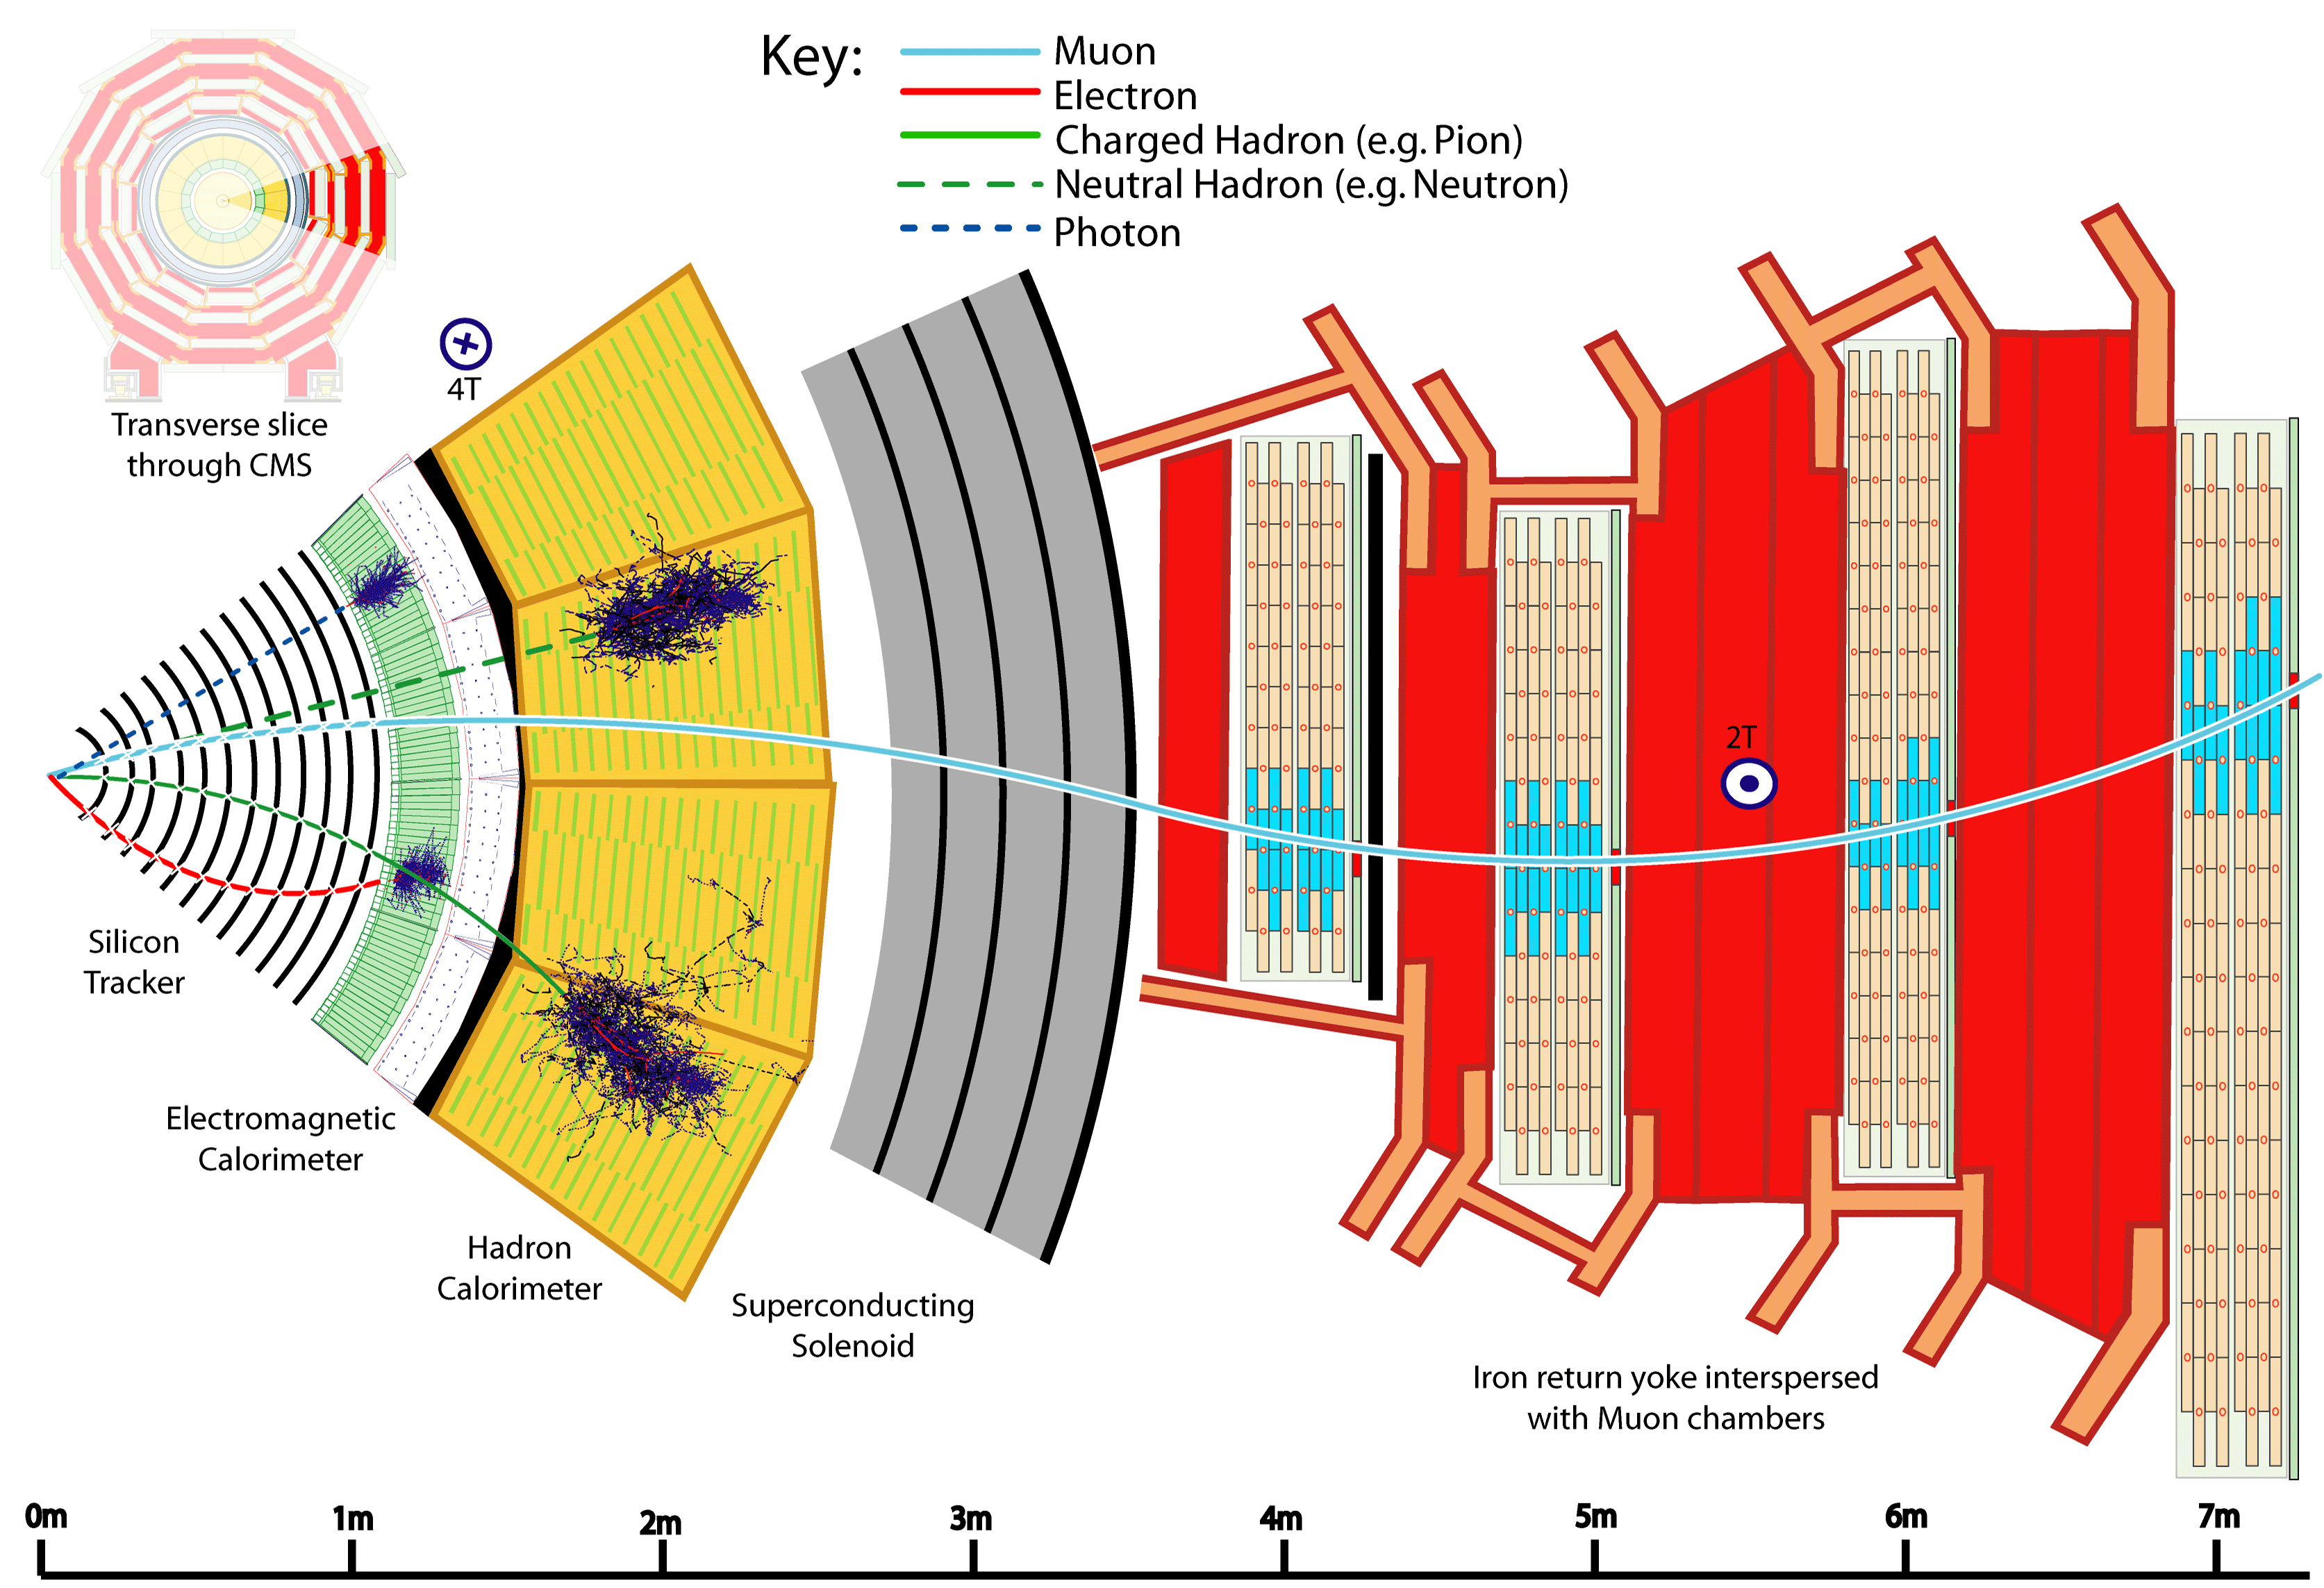
\includegraphics[angle=-0,width=0.8\textwidth]{2_LHC_and_CMS/pics/CMS_Slice_HD.png}
\caption{Schematic view of a slice of the barrel of the CMS detector and the path travelled by different kind of particles with the signal deposed in each subdetector.
\label{fig:cmsdet}
}
\end{center}
\end{figure}


\subsection{Coordinate system}
The coordinate system chosen for CMS sets the $y$ axis vertical pointing upwards and the $x$ axis horizontal pointing towards the center of LHC, therefore the $z$ axis is placed along the beam line pointing in the direction of the beam running anti-clockwise or towards the Jura. An additional set of polar coordinates is used to describe the $xy$ plane in the form of radius $r$ and angle $\phi$, while the angle $\theta$ is measured with respect to the positive $z$ axis direction. Usually the angle $\theta$ is replaced by the \emph{pseudorapidity} defined as $\eta=-\ln \tan(\theta/2)$ that has the property to be a Lorentz invariant for boosts along the $z$ axis and therefore comes very handy when describing processes whose longitudinal boost is unknown. The three-dimensional angular distance is also replaced by its lorentz-invariant which is $\D R=\sqrt{\D\phi^2+\D\eta^2}$.

\subsection{Inner Tracker}

The inner tracker provides the essential spatial informations needed to reconstruct charged tracks and primary and secondary vertices. A schematic view of the inner tracker is depicted in figure \ref{fig:tracker}. To cope with the very high occupancy and to provide the best possible spatial resolution the innermost part of the tracker exploits silicon pixel technology. The pixel detector, whose design scheme is reposted in figure \ref{fig:pixel}, is composed of three cylindrical layers set at radii of 4.4, 7.3 and 10.2 cm complemented by four disks  in the forward/backward region. The total active area of the pixel detector is roughly of 1m\sq~and its acceptance covers up to $|\eta|$ of 2.5, providing 3 bi-dimensional measurements over the full acceptance. The pixel cell size is 100 $\times$ 150 \u m\sq. The ionization charge is shared between neighboring pixels due to the immersion of the sensors in the solenoidal magnetic field. To enhance this effect in the forward wheels the sensors are placed in a turbine shape. Pulse shape analogue read-out and charge sharing allow for a 15-20 \u m resolution. 

The pixel detector is mechanically decoupled from the rest of the tracker to allow easy access for maintenance without interfering with the rest of the detector. This feature is particularly important due to the high radiation dose that the first layers of the pixel detector sustain, requiring additional maintenance.

\begin{figure}
\begin{center}
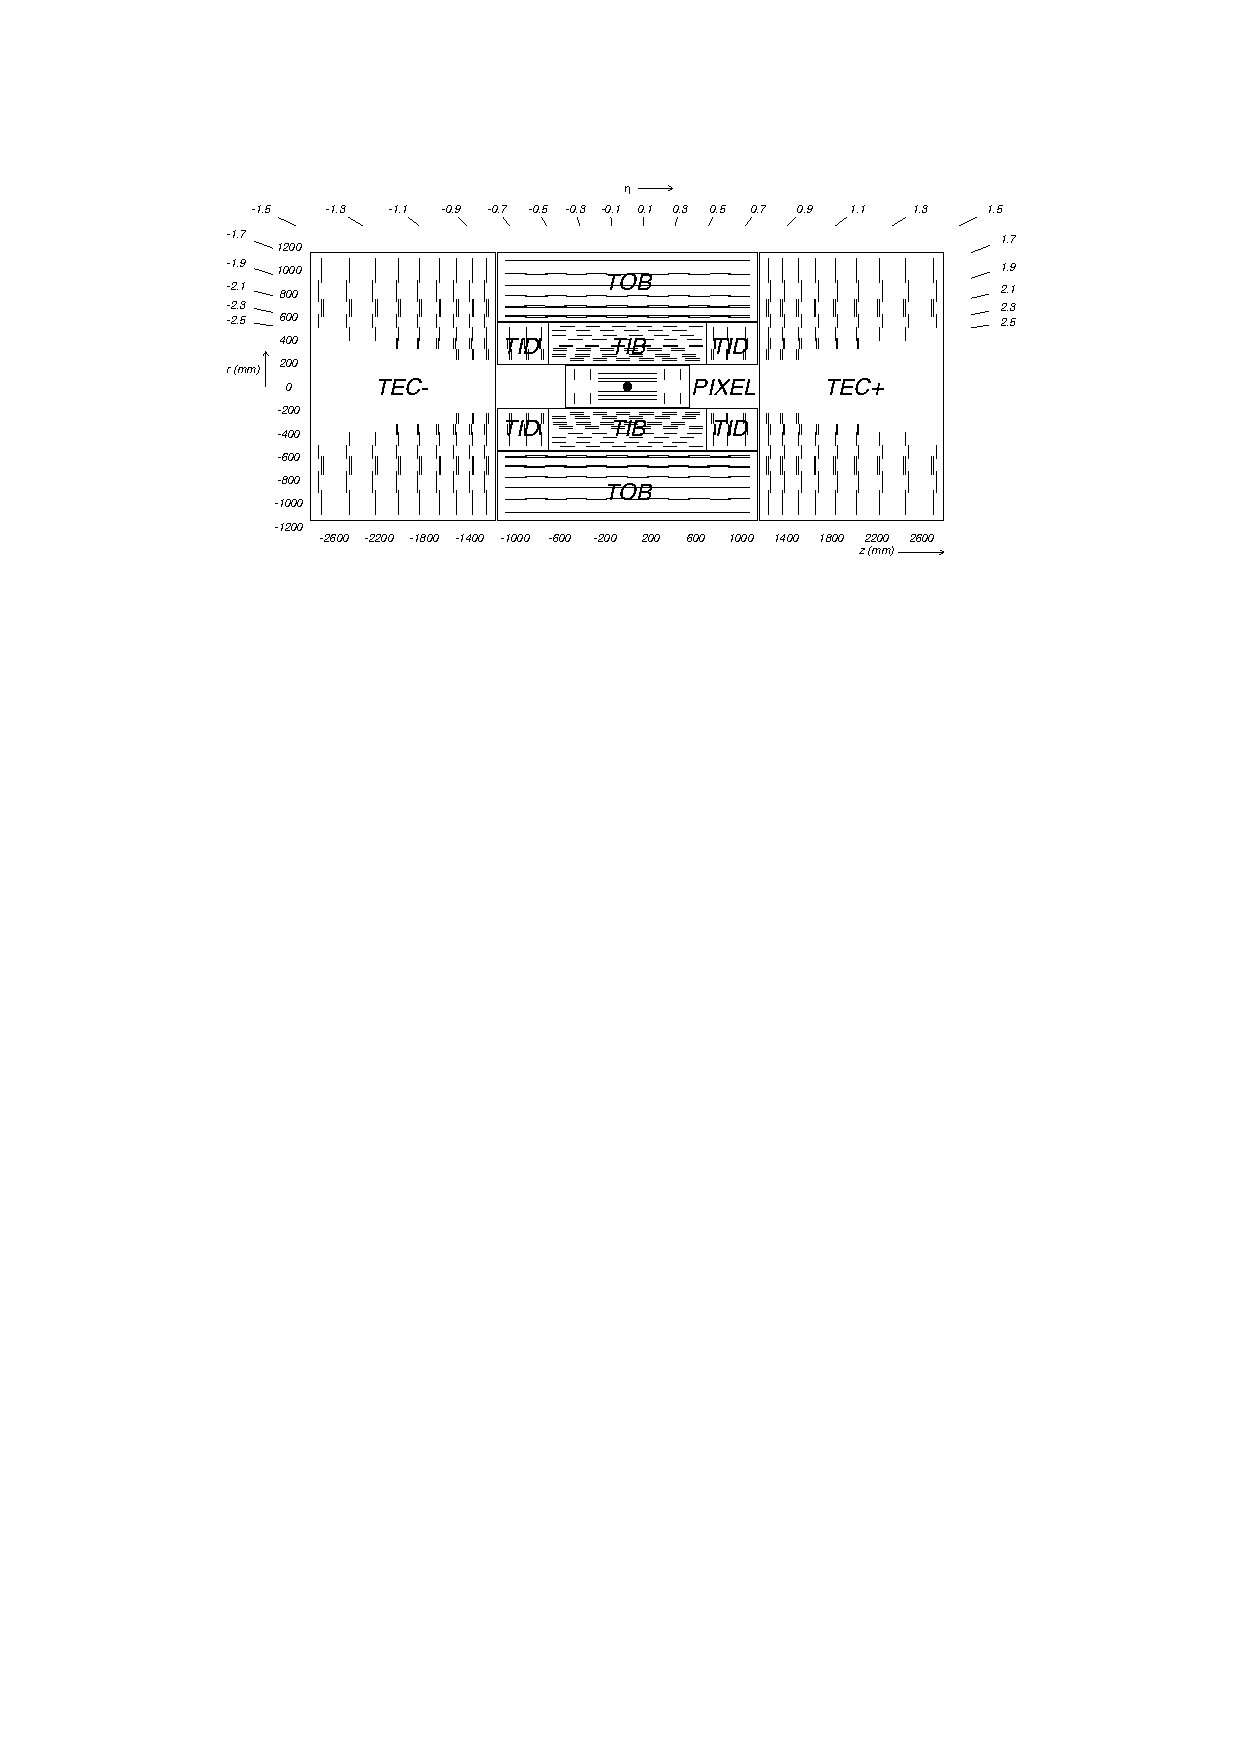
\includegraphics[angle=-0,width=0.8\textwidth]{2_LHC_and_CMS/pics/trkxsec.pdf}
\caption{Longitunal cross section of the CMS tracker with pseudo rapidity coverage. 
\label{fig:tracker}
}
\end{center}
\end{figure}

\begin{figure}
\begin{center}
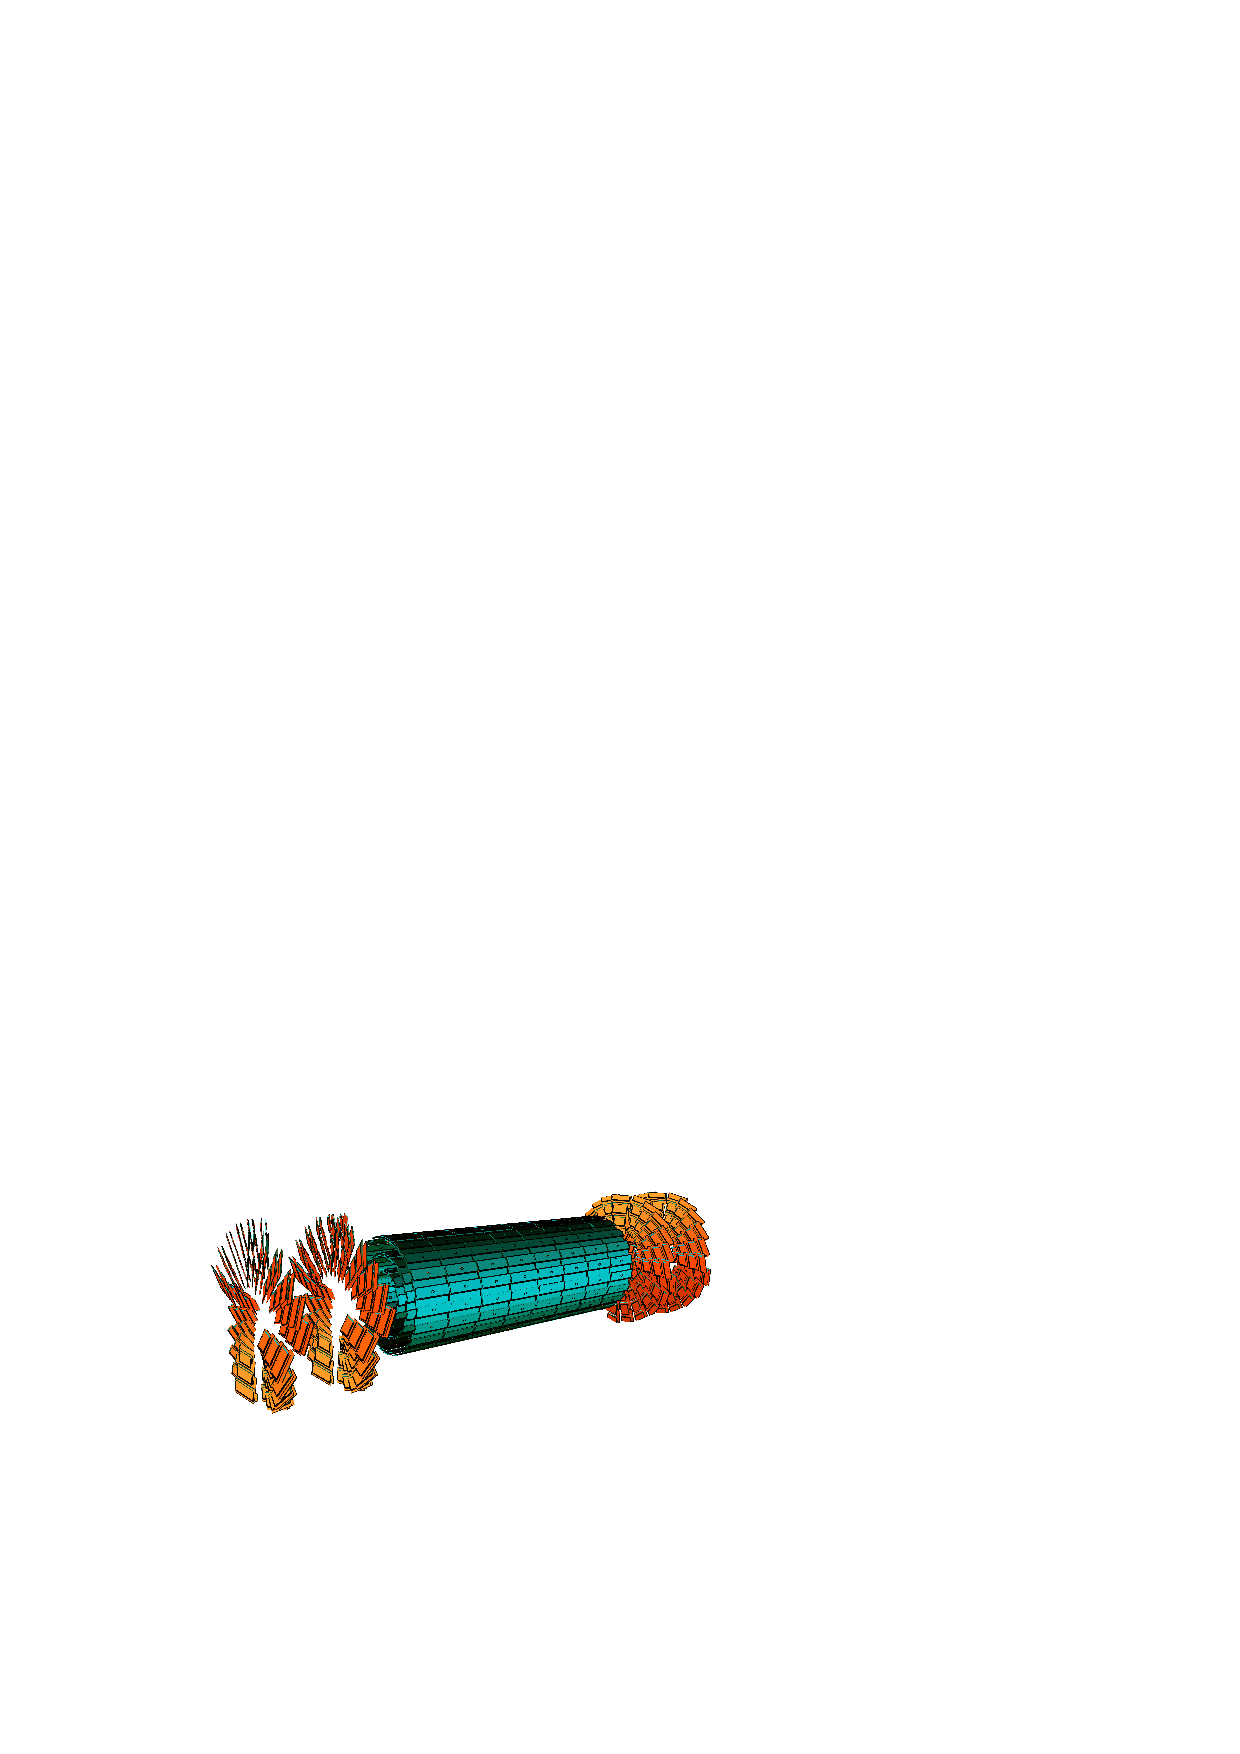
\includegraphics[angle=-0,width=0.8\textwidth]{2_LHC_and_CMS/pics/pixelfull.pdf}
\caption{Three dimensional sketch of the CMS pixel detector, barrel modules in blue and end cap wheels in orange.
\label{fig:pixel}
}
\end{center}
\end{figure}

On the outer layer the tracker is made of silicon strip detectors and furtherly divided into four parts: Tracker inner/outer barrel (TIB and TOB), tracker inner disks (TID) and tracker end-caps (TEC). TIB and TID are located between 20 and 55 cm in radius from the beam line. They consists of four barrel layers and three disks at each end. The sensors are made of 320 \u m thick silicon with a strip pitch that varies from 80 \u m of the innermost barrel layer to 140 \u m of the outermost disks. The combination of TIB and TID delivers up to four $r-\phi$ measurements. The TIB/TID is surrounded by the TOB, which fills the remaining space up to a radius of 116 from the beam line. It consists of six barrel layers of 500 \u m thick sensors with a strip pitch of 183 \u m for the first four layers and 122 \u m for the remaining two. The TEC is located in the end-cap region, for radii greater than 20 cm and $|z| > 118$ cm. The TEC consist in nine disks composed by up to seven concentric rings of strip sensors. The thickness and the strip pitch of the sensor varies depending on the distance of the ring from the beam line. 

Intrinsically strip sensors only provide one dimensional measurement ($\phi$), to achieve the measurement of the second coordinate ($r$ for disks, $z$ for barrel) an additional set of sensors is mounted back to back with a stereo angle of 100 mrad on the first two layers of TIB, TID and TOB and on layers 1, 2 and 5 of TEC. This layout ensures \~9 hits in the strip tracker in the full acceptance with at least four of them being bi-dimensional.

%temperatura?

\subsection{ECAL}

The CMS electromagnetic calorimeter (ECAL) is located around the inner tracker. It is divided into ECAL Barrel (EB) covering the pseudo rapidity range of $|\eta| < 1.479$ and ECAL Endcaps (EE) which covers up to 3 in pseudo rapidity both in the forward and backward region. 
The calorimeter consist of 68524 scintillating lead tungstanate (PbWO$_4$) crystals read-out by photomultipliers. 

The choice of lead tungstanate was driven by its high density yielding a short radiation length (0.89 cm) and small Moliere radius (2.2 cm) together with the radiation hardness and fast response, 80\% of the light yield is in fact emitted in 25~ns. To keep the calorimeter as hermetic as possible the crystals have truncated pyramidal shape with one of the longitudinal faces left unpolished to moderate the non uniform light collection across the crystal length that this peculiar shape causes. Each crystal covers about $0.0174 \times 0.0174$ in $\eta-\phi$ plane and is oriented pointing towards the nominal interaction point with a slight misalignment to mitigate the effect of the crystal surface on photon detection. Each crystal is read-out by either a pair of Avalanche Photodiodes (APD) in the barrel or by vacuum phototriodes in the end cap. Both the devices can operate in high magnetic fields with little or no efficiency degradation. 

A pre-shower detector is housed in front of the ECAL end cap, with the purpose of discriminating between real photons and in-flight decays of \piz and to enhance the angular resolution of both electrons and photons. The pre-shower detector consist in a double-layer lead-silicon calorimeter, with the lead initiating the shower and the silicon strip detector placed after each radiator measuring deposited energy and shower profile with high granularity.

\subsection{HCAL}

The hadronic calorimeter (HCAL) serves two purposes: measures the energy of charged and neutral hadrons coming from the interaction point while stopping them, thus allowing only muons to pass through and avoiding large quantities of energy being deposited inside the superconducting magnet. As of most the other detectors HCAL is divided in a barrel (HB), covering the acceptance region of $|\eta| < 1.3$, and an end cap (HE) which brings the acceptance up to $|\eta| < 3$. Both parts are located inside the superconducting solenoid. HCAL is a sampling calorimeter with brass passive plates, in which the hadronic shower begins and develops, interspaced with active plastic scintillator material recording the shower development. 

The scintillator is segmented both in $\eta$ and in $\phi$ to provide the required granularity. Each scintillating tile is connected to the read-out by a wavelength-shifting fiber that runs in a groove machined in the tile itself. Such fiber is thermally spliced to a clear fiber carrying the emitted light to a hybrid photodiode (HPD). HPD's consist of a photocathode kept at high voltage. Electrons emitted by the photocathode are accelerated in the short distance (\~3 mm) that separates the cathode from a silicon pixelated anode which amplifies the signal. These devices were chosen due to their high dynamic range, their high gain ($O(2000)$) and the possibility to work in a magnetic field.

The effective thickness of the calorimeter in terms of interaction length ($\lambda_I$) spans in the barrel from a minimum of 5.82 $\lambda_I$ at $\eta=0$ to a maximum of 10.6 $\lambda_I$ at $|\eta| = 1.3$. The ECAL crystals add about 1.1 additional interaction lengths. The total thickness of the end cap calorimeters, including in the ECAL crystals, is about 10 $\lambda_I$.

Due to the limited stopping power of HB, especially in the central rapidity region, an additional hadronic calorimeter is placed outside the solenoid magnet (hadron outer or HO) with the function of \emph{tail catcher}. HO consist of one scintillating station (two for the most central region) exploiting the solenoid itself ( and the first return yoke in case of the second station) as absorber. This additional detector extends the total thickness of the HB up to a minimum of $11 \lambda_I$.

\subsection{Muon System}

Muon detection and trigger is of prime importance as of many new physics processes may become manifest through decay chains involving muons. Among those the decay of a Higgs boson into $ZZ^*\To4\mu$ stands out as one of CMS's flagship analyses and one of those which led to the discovery of the Higgs boson announced on the 4$^{th}$ of July 2012. For this reason a redundant system of three different kinds of detectors is used to track muons in CMS. 

The muon system, whose scheme can be found in figure \ref{fig:mudet} is housed in gaps between the return yoke of the solenoid magnet in the outermost region from the nominal interaction point. It consists of a Drift Tube (DT) tracking system in the barrel and multi-wire proportional chambers in the end-cap. In addition to these two detectors a set of Resistive Plate Chambers (RPC) is located both in the barrel and in the end cap, providing a better time resolution  at the cost of coarser spatial resolution. 

\begin{figure}
\begin{center}
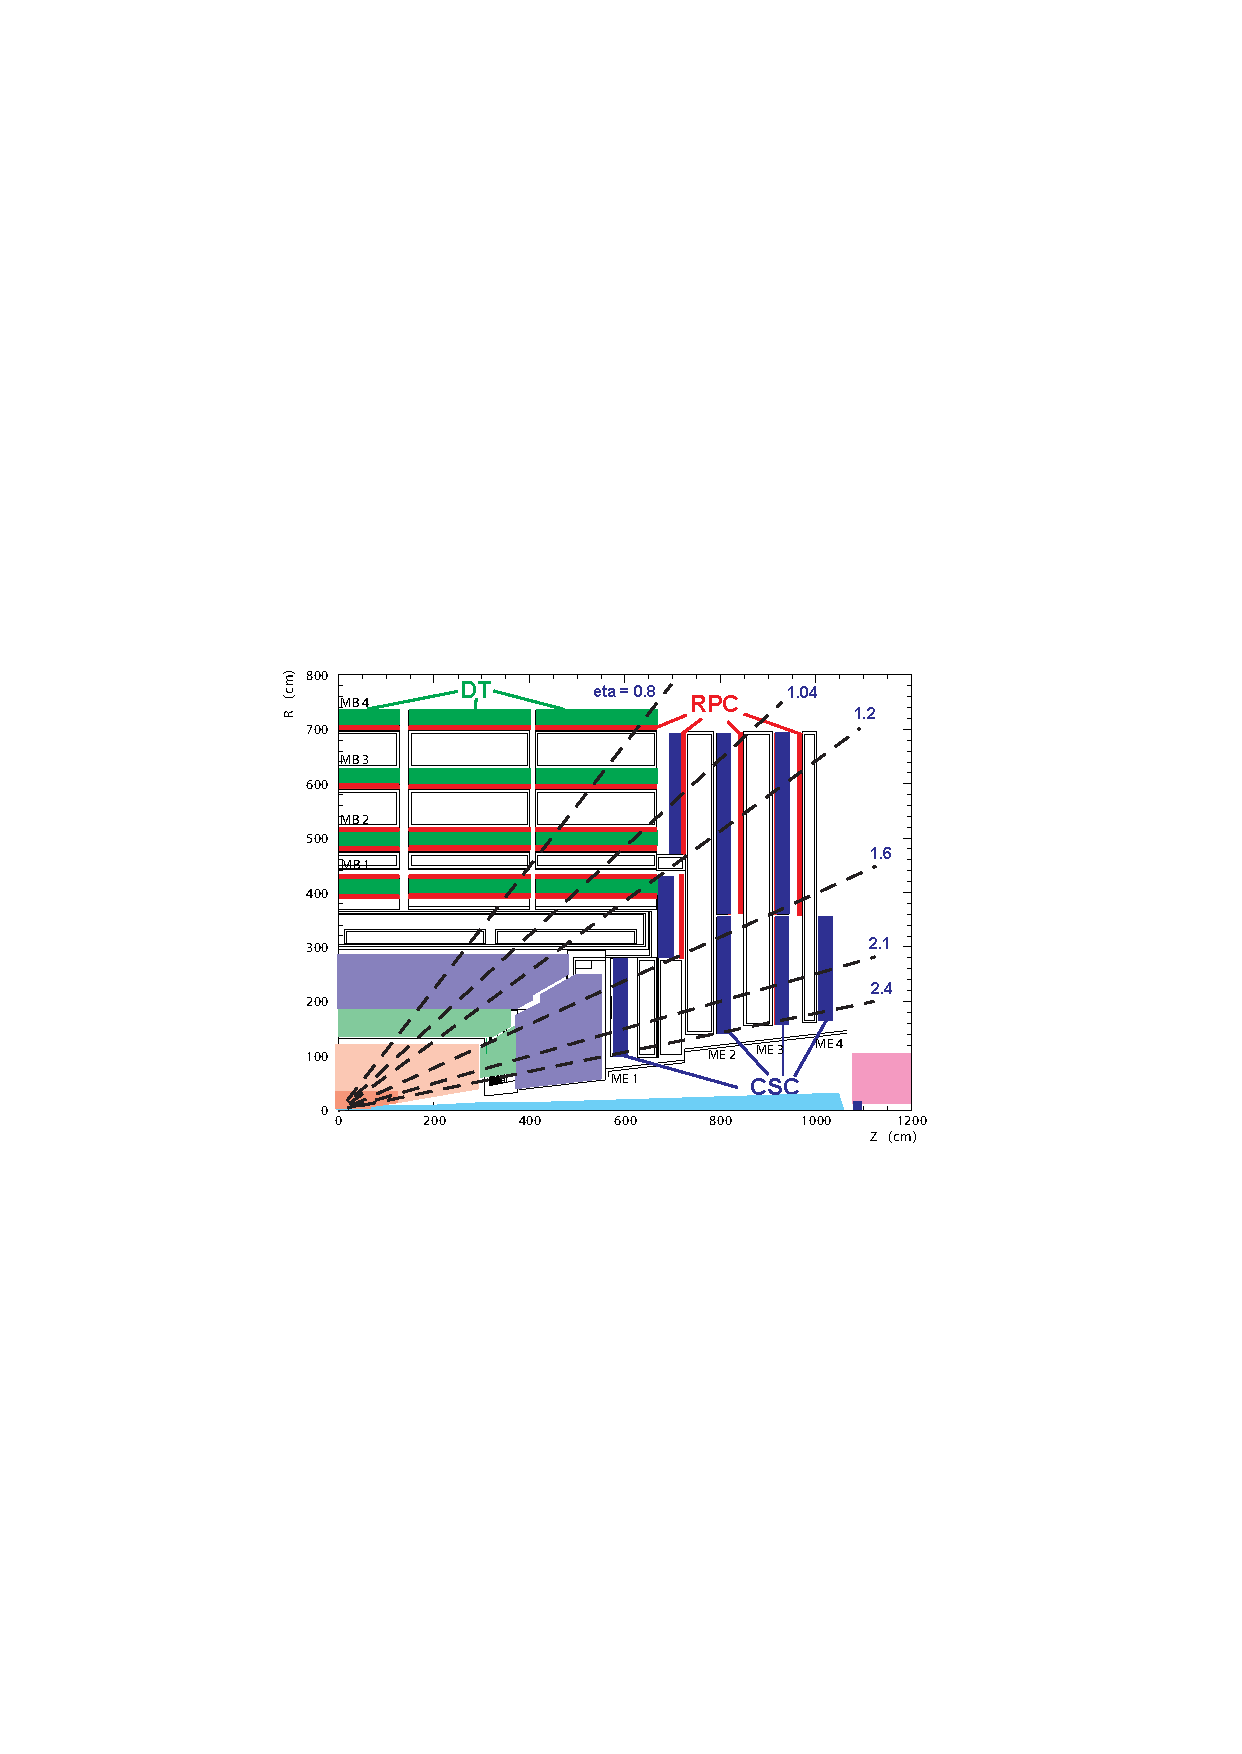
\includegraphics[angle=-0,width=0.8\textwidth]{2_LHC_and_CMS/pics/mudet.pdf}
\caption{Longitudinal cross-section of the CMS detector showing the location of the muon system.
\label{fig:mudet}
}
\end{center}
\end{figure}

\subsubsection*{Drift Tubes}

Drift tubes take care of muon tracking in the barrel region ($|\eta| < 1.2$) where muon rate less than 1 Hz/cm\sq ~and residual magnetic field less than 1 T make feasible the use of this technology. Four station are located at increasing distance from the beam line. The first three stations are equipped with two \emph{super-layers} (SL) providing a measurement of $\phi$ and one SL measuring the $z$ coordinate as can be seen in figure \ref{fig:dt_module} representing one DT module. In the last two stations the SL measuring the $z$ coordinate is missing. 

\begin{figure}
\begin{center}
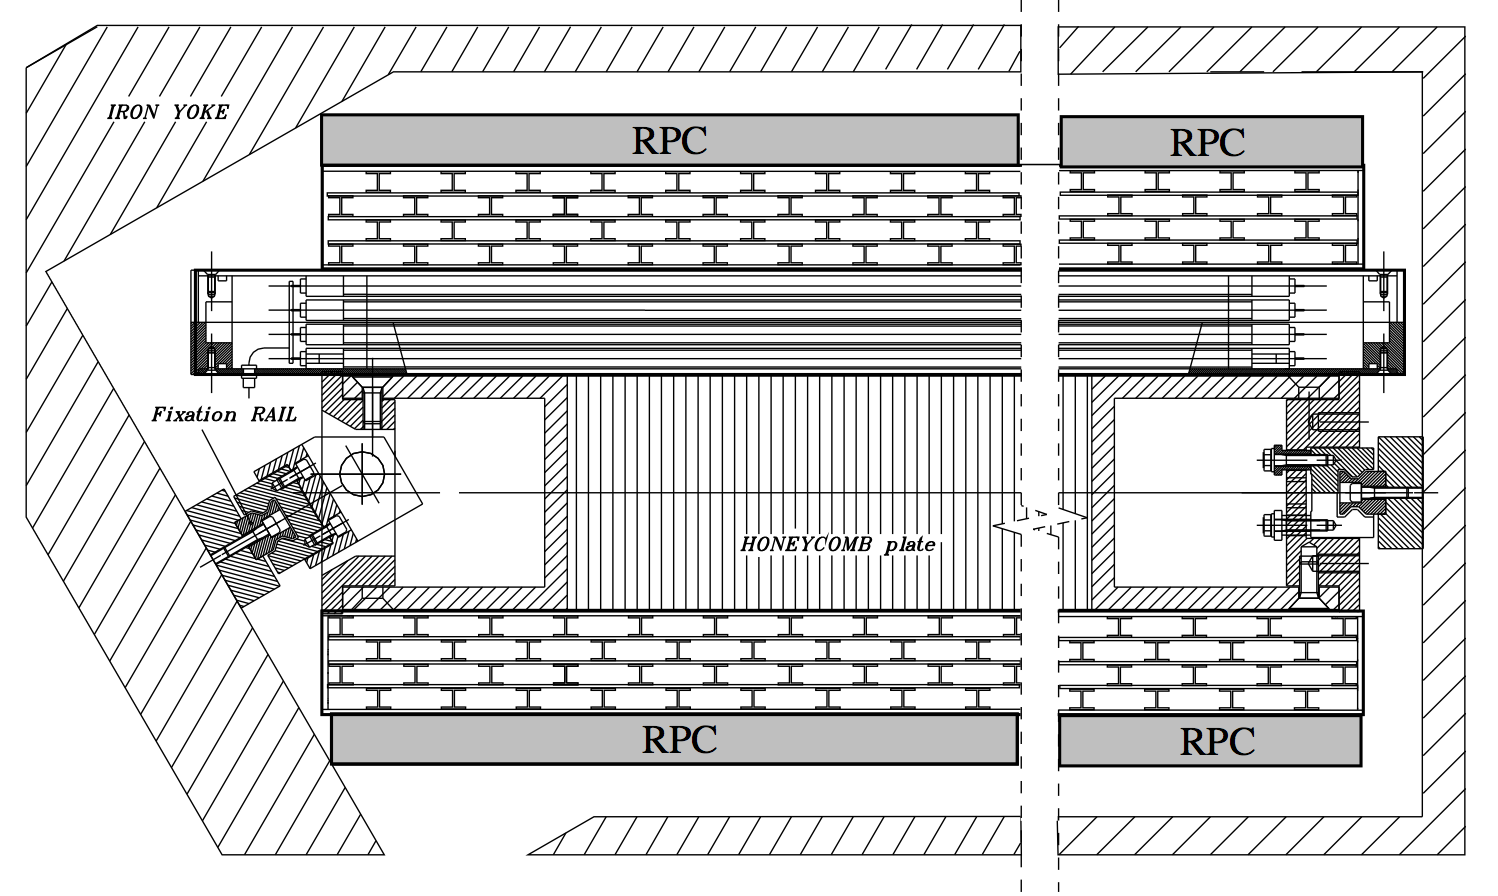
\includegraphics[angle=-0,width=0.8\textwidth]{2_LHC_and_CMS/pics/cms_dt.png}
\caption{Cross-section view of a DT module.
\label{fig:dt_module}
}
\end{center}
\end{figure}


Each SL is made of four stacked layers of tubes staggered by half a cell. This configurations eliminates blind spots and allow for an easy measurement of the muon passing time by averaging the drift times. Each tube has rectangular a cross-section of $13\times42$ mm\sq ~and is filled with a gas mixture of 85\% Ar and 25\% CO$_2$ leading to a maximum drift time of 380 ns. Each SL has a spatial resolution of about 200 \u m and a jitter smaller than 5 ns.

\subsubsection*{Cathode Strip Chambers}

The front wheels of the solenoid return yoke are instrumented with multi-wire proportional chambers. Each module has trapezoidal shape and cover either $10\deg$ or $20\deg$ in $\phi$ forming a full disk perpendicular to the beam axis ($r-\phi$ plane). Each of these chambers has the cathode segmented radially in strips (hence the name Cathode Strip Chamber, CSC) of constant $\Delta\phi$ and wires running perpendicular to the strips with spacing of 3.2 mm. 

This design allows to cope with the much higher rate with respect to the barrel and with non uniform and non null magnetic field. 

This detector provides at least three measured point in its acceptance ($1.2 < |\eta| < 2.4$) with a design resolution of approximately 2 mm at trigger level and around 200 \u m offline.

\subsubsection*{Resistive Plate Chambers}

Dual-gap RPC's provide a redundant set of spatial measurements particularly important for trigger purposes, given their response time much shorter than 25~ns. The layout chosen by the CMS collaboration consist of six RPC stations in the barrel and three in the end caps. RPC stations are placed in proximity (before or after) each CSC or DT station. The first two DT station have two RPC, one before \emph{and} one after, in order to provide at least four position measurements even for low-$p_T$ muons which might not reach the outer stations. Each chamber is operated in avalanche mode and consist of two gaps sharing a segmented pick-up read-out in between, allowing to operate at lower voltages (and therefore lower noise) for the same gain. 

\subsection{Trigger}

The bunch crossing frequency of 20 MHz delivered by LHC is well above the storage capabilities of the most modern technologies allowing to accommodate few hundreds of events per second. It is also true looking at figure 
\ref{fig:sm_xsec} %da mettere nel capitolo 1 - xsection SM
that the inclusive p-p cross-section is hugely dominated by low-$x$ QCD processes that are of no or little interest for this experiment leading to the obvious necessity of a fast-logic to isolate events of some interest for the experiment's physics program while rejecting the others. This kind of logic, usually referred as \emph{trigger}, is divided in the CMS experiment in two stages: the \emph{level one} (L1) trigger and the \emph{high level trigger} (HLT). 

The L1 trigger decision is based on a coarse reconstruction of the event performed by custom electronics largely mounted directly on the detector. The maximum processing time (called \emph{latency}) is 3.2 \u s, in this time the event stays stored on the detector electronics in pipelined memories. Due to timing constraints only inputs from the calorimeters and from the muon system are processed. For the purpose of triggering the calorimeter segmentation is reduced into the so-called \emph{trigger-towers}. Calorimeters provide to the decision logic a set of important physics variables like $E_T^{miss}$, scalar sum of the transverse hadronic activity ($H_T$), number of jets above different thresholds and locations of towers compatible with a \emph{minimal ionizing particle} (MIP) and its isolation. An electron and photon identification is also performed looking at the jet hadronic over electromagnetic energy ratio ($H/E$) and cluster shape, performed with the aid of a look-up table. Muon information is mainly provided by DT and CSC sub-detectors complemented by the sheer time resolution of RPC for bunch crossing assignment as well as ghost-tracks removal. Muons trajectories are roughly reconstructed inside the detector's dedicated electronics and then sent to an additional module that merges the information coming from the different stations and sub-detectors assessing the transverse momentum  and charge. These informations are complemented by the ones coming from the calorimeters providing isolation values.

The final decision is taken by modules located outside the detector. These modules exploit the FPGA technology to achieve fast response while still allowing for modification of the algorithms as the instantaneous luminosity conditions evolve, or if new physics demands are posed. The maximum output frequency for L1 was chosen to be 1kHz.

Once the L1 trigger decision is made the full event is read from the detectors buffers and sent to the online \emph{Data Quality Monitoring} (DQM) and to the HLT farm, consisting of over a thousand commercial processor working in parallel. During the HLT decision making a more simple and coarse version of the full CMS reconstruction is performed. Time consuming task like tracking are performed only around the objects that caused the L1 trigger to fire and complex algorithms like \b-tagging and \t~identification are performed with a simplified version. During this trigger stage decision are taken based on more complex algorithms and a more refined reconstruction allowing to reduce the event rate to roughly 100Hz, which is within the capabilities of storage of CMS and CERN facilities. Beeing completely software, the HLT is far more flexible and fast evolving than L1 trigger allowing to cope with the fast changing machine conditions during 2010 and 2011 runs and to achieve a level of refinement beyond the most optimistic forecasts made at the start-up.

Once the event is also accepted by the HLT is transferred to the above ground facilities for storage and reconstruction.

\section{Data storage and processing}

Reconstruction of data collected by the experiment as well as the full simulation of interesting physics processes are too CPU and storage demanding to be delegated to a single facility. In order to evenly spread this effort through different computing facilities in various parts of the world, a new computing model was created. The \emph{world wide computing grid} allows for fast transfer and de-localized computing throughout the world, allowing to cope with the huge demands that the LHC experiments need to smoothly operate. 

In some sense the grid can be seen as an extension of the batch queue system where the user submit his jobs to a single machines, whereas in this case he submits them to clusters of machines, that then take care of submitting those jobs in their peculiar batch queue scheduler implementation. Computing facilities are organized in a hierarchical structure called tiers, starting from the facility that receives the data from the detector called Tier0, scaling to smaller and smaller facilities up to Tier3's providing limited computing and storage for local groups while still being connected to the grid and therefore profiting of the fast transfer abilities. In this system secure access to the resources is ensured by a system of certificates spawning children proxies of limited lifetime.

